\item[(a)]
	\begin{itemize}  
	\item[i.]	
	For one vs. all, there are \textbf{k} classifiers because each label will generate one classifier and there are k labels.\\
	For all vs. all, there are \textbf{k(k-1)/2} classifiers because each pair of labels will generate one classifier and there are $C^k_2=k(k-1)/2$ pairs of labels. 
	\item[ii.]
	For one vs. all, number of positive examples is m/k and number of negative examples is m(k-1)/k for each classifier. Total number of examples used to learn is \textbf{m}.\\
	For all vs. all, number of positive examples is m/k and number of negative examples is m/k for each classifier.
	Total number of examples used to learn is \textbf{2m/k}. 
	\item[iii.]
	For one vs. all, there are k classifiers corresponding to k labels. The input example will be labeled i if the $i_{th}$ classifier returns positive.
	For all vs. all, every pair, $\langle i, j \rangle$, has its own classifier. If the example is labeled by all classifiers $\langle i, j \rangle, j\in [1,2,...,k], j\not= i$ as i, the example is thought to be in i.
	\item[iv.]
	For one vs. all, there are k classifiers with m training examples for each, so $O(km)$.\\
	For all vs. all, there are k(k-1)/2 classifiers with 2m/k training examples for each, so $O(k(k-1)/2\times 2m/k)=O(km)$.
	\end{itemize}
\item[(b)]
All vs. all.\\
According to the analysis above, both method achieve the same computational complexity. However, it is possible that sets between all pairs of labels are linear separable but not separable when considering the set of one label to the union set of all other labels. If that happens, all-vs-all method can classify the examples well, but one-vs-one method cannot. For example, there are 3 sets of examples in 3 labels shown in figure. Using one-vs-all method is impossible to find a linear classifier telling the set in red. On the other hand, using all-vs-all method, all pairs of sets are linear separable generating corresponding classifiers telling each pair of sets. The examples can be classified correctly. Thus, all vs. all is a better choice.\\
\begin{figure}[h]
		\centering
	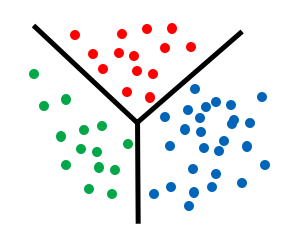
\includegraphics[width=0.4\textwidth]{fig3.png}
\end{figure}\\\\

\item[(c)]
A \textsc{KernelPerceptron} can extend the space of the examples into another space in higher order and possibly separate the examples in the new space. Considering the same linear separability issue in the higher order space as we had in (b), all-vs-all method will outperform one-vs-one method. Besides, kernel functions should work in dual mode because most of kernel functions cannot find a transfer function from original space to the higher order space, but can calculate the inner product of two vectors. That means the computational complexity of these two methods when classifying is proportional to the training examples and the number of the classifiers. Thus, the computational complexity for one-vs-all method is $O(mk)$ and the computational complexity for all-vs-all method is $O(k(k-1)/2\times 2m/k)=O(km)$. Thus, after considering performance and complexity, I still choose all vs. all.

\item[(d)]
For one vs. all, there are k classifiers with m training examples to learn. The computational complexity is $O(kdm^2)$.
For all vs. all, there are k(k-1)/2 classifiers with 2m/k training examples to learn. The computational complexity is 
$O(\frac{k(k-1)}{2}d(\frac{2m}{k})^2) = O(dm^2)$. All vs. all is most efficient.

\item[(e)]
For one vs. all, there are k classifiers with m training examples to learn. The computational complexity is $O(kd^2m)$.
For all vs. all, there are k(k-1)/2 classifiers with 2m/k training examples to learn. The computational complexity is 
$O(\frac{k(k-1)}{2}d^2(\frac{2m}{k})) = O(kd^2m)$. Both are the same in efficiency.

\item[(f)]
It takes $O(d)$ to calculate $w^T_ix$. For \textbf{Counting}, it takes $O(d\times k(k - 1)/2)= O(dk^2)$ because all k(k - 1)/2) classifiers should be calculated.
For \textbf{Knockout}, after (k-1) comparisons, there will be only one label left which means the end of the classification. Thus, total number of comparisons is k-1. It takes $O(d\times (k-1))=O(dk)$.  





